\chapter{De la graine à la plante}\label{ch:g2:from-seed-to-plant}

Secoue une cosse de haricots séchée et de petits haricots durs en
tombent --- secs, ternes, apparemment aussi inertes que du gravier.
Pourtant, plantes-en un dans la terre et arrose-le~: en quelques
jours, quelque chose d'extraordinaire se passe sous le sol. Toute une
\omterm{def:g1:plants-around-us:plant}{plante} était pliée à l'intérieur, en attente de son signal.

\section{Ce qu'est une graine}

\begin{definition}[Graine]\label{def:g2:from-seed-to-plant:seed}
Une \emph{graine}\index{graine} est le commencement d'une nouvelle
\omterm{def:g1:plants-around-us:plant}{plante}, fabriqué par la \omterm{def:g1:plants-around-us:plant}{plante} mère. Sous son enveloppe protectrice,
une graine contient~:
\begin{itemize}
  \item une toute petite \omterm{def:g1:plants-around-us:plant}{plante} déjà commencée --- le
        \emph{germe}\index{germe (de la graine)} de la \omterm{def:g1:plants-around-us:plant}{plante}, avec
        le début d'une \omterm{def:g1:plants-around-us:parts}{racine} et d'une \omterm{def:g1:plants-around-us:parts}{tige}~;
  \item une réserve de nourriture pour la nourrir jusqu'à ce
        qu'elle puisse se nourrir seule.
\end{itemize}
\end{definition}

\begin{example}[Ouvrir un haricot trempé]\label{ex:g2:from-seed-to-plant:open}
Fais tremper un gros haricot blanc toute une nuit~: son enveloppe se
retire toute seule. Le haricot s'ouvre en deux moitiés épaisses ---
la réserve de nourriture --- et là, blottie sur un bord, se trouve
une toute petite \omterm{def:g1:plants-around-us:plant}{plante} pâle, pointe de \omterm{def:g1:plants-around-us:parts}{racine} et premières \omterm{def:g1:plants-around-us:parts}{feuilles}
pliées, grosse comme un grain de riz. La nouvelle \omterm{def:g1:plants-around-us:plant}{plante} était là
depuis le début.
\end{example}

\begin{omfigure}
\begin{tikzpicture}
  \node[anchor=south west, inner sep=0] (img) at (0,0)
    {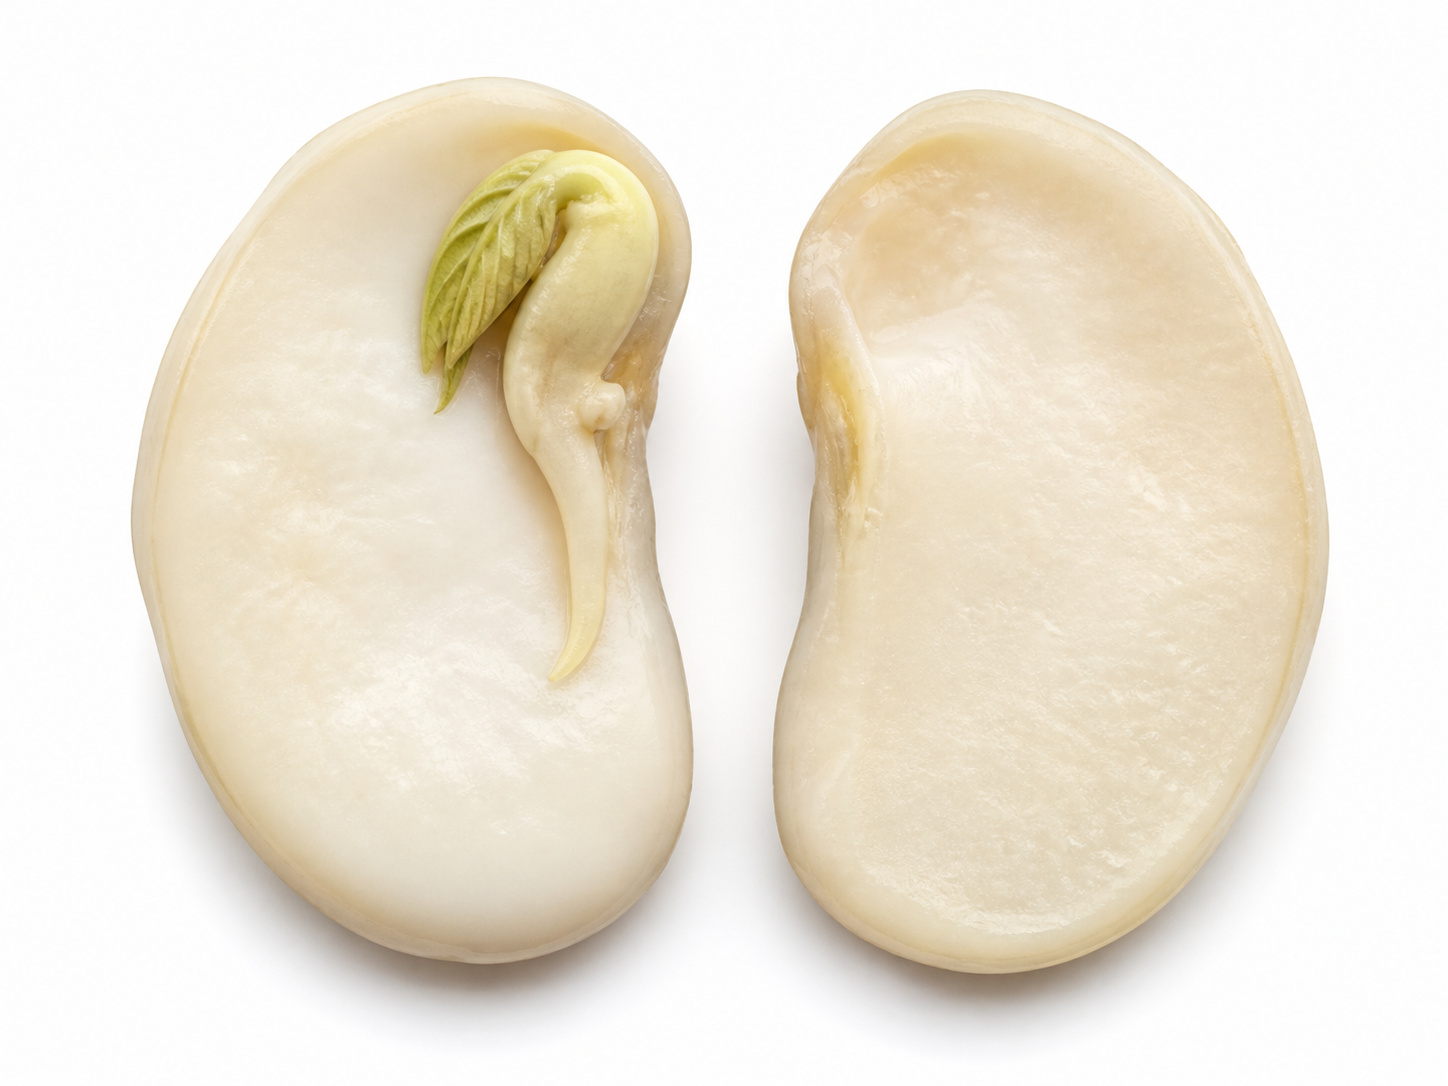
\includegraphics[width=0.62\linewidth]{images/book1/ai/fig-bean-open.png}};
  \begin{scope}[x={(img.south east)}, y={(img.north west)},
      every node/.style={font=\small}]
    \draw[omDef, thick] (0.35,0.79) -- (0.26,0.94)
      node[above] {les premières feuilles pliées};
    \draw[omDef, thick] (0.40,0.38) -- (0.28,-0.04)
      node[below] {la pointe de la racine};
    \draw[omDef, thick] (0.78,0.35) -- (0.80,-0.04)
      node[below, align=center] {les deux moitiés épaisses~:\\ la réserve};
  \end{scope}
\end{tikzpicture}

{\small À l'intérieur du haricot trempé et ouvert~: une toute petite
\omterm{def:g1:plants-around-us:plant}{plante} --- pointe de \omterm{def:g1:plants-around-us:parts}{racine} et premières \omterm{def:g1:plants-around-us:parts}{feuilles} pliées ---
couchée contre sa réserve de nourriture.}
\end{omfigure}

\begin{remark}[Des graines passent par nos cuisines]\label{rem:g2:from-seed-to-plant:kitchen}
Haricots, pois, lentilles, riz, \omterm{def:g2:from-seed-to-plant:seed}{graines} de tournesol, pépins de la
pomme et noyau de la pêche~: la cuisine est pleine de \omterm{def:g2:from-seed-to-plant:seed}{graines}.
Certaines sont minuscules, comme les \omterm{def:g2:from-seed-to-plant:seed}{graines} de pavot~; la noix de
coco en est une géante. Chacune, si on lui en laissait l'occasion,
essaierait de devenir une \omterm{def:g1:plants-around-us:plant}{plante}.
\end{remark}

\section{La germination}

\begin{definition}[Germination]\label{def:g2:from-seed-to-plant:germination}
La \emph{germination}\index{germination} est le moment où une \omterm{def:g2:from-seed-to-plant:seed}{graine}
se réveille et se met à pousser~: elle gonfle d'eau, son enveloppe se
fend, la petite \omterm{def:g1:plants-around-us:parts}{racine} sort la première et plonge vers le bas, puis
la \omterm{def:g1:plants-around-us:parts}{tige} s'élève, portant les premières \omterm{def:g1:plants-around-us:parts}{feuilles} vertes vers la
lumière. On dit que la \omterm{def:g2:from-seed-to-plant:seed}{graine} \emph{germe}\index{germer}.
\end{definition}

\begin{proposition}[Ce qu'il faut à une graine pour germer]\label{prop:g2:from-seed-to-plant:needs}
Pour \omterm{def:g2:from-seed-to-plant:germination}{germer}, une \omterm{def:g2:from-seed-to-plant:seed}{graine} a besoin d'\emph{eau} et de \emph{chaleur}.
Elle n'a pas encore besoin de lumière~: la réserve nourrit d'abord la
\omterm{prop:g2:from-seed-to-plant:cycle}{jeune pousse}, même sous la terre, dans le noir. Sans eau, ou dans le
froid, une bonne \omterm{def:g2:from-seed-to-plant:seed}{graine} se contente d'attendre.
\end{proposition}
\admitted

\begin{example}[Pourquoi les semis attendent le printemps]\label{ex:g2:from-seed-to-plant:spring}
Les jardiniers sèment les haricots au printemps, pas en hiver~: dans
une terre froide, la \omterm{def:g2:from-seed-to-plant:seed}{graine} attendrait --- ou pourrirait --- au lieu
de \omterm{def:g2:from-seed-to-plant:germination}{germer}. Des journées douces et un sol arrosé sont exactement les
deux signaux de \cref{prop:g2:from-seed-to-plant:needs}.
\end{example}

\begin{method}[Semer une graine et regarder germer]\label{met:g2:from-seed-to-plant:sow}
\begin{enumerate}
  \item Tapisse un bocal en verre de coton ou de papier humide~;
  \item glisse un haricot entre le verre et le coton, pour bien le
        voir~;
  \item garde le bocal dans une pièce chaude et le coton humide~;
  \item regarde chaque jour et note ce que tu vois~: le gonflement,
        l'enveloppe qui se fend, la \omterm{def:g1:plants-around-us:parts}{racine} vers le bas, la \omterm{def:g1:plants-around-us:parts}{tige} vers
        le haut.
\end{enumerate}
Le verre rend visible ce qui se passe d'habitude sous la terre.
\end{method}

\begin{omfigure}
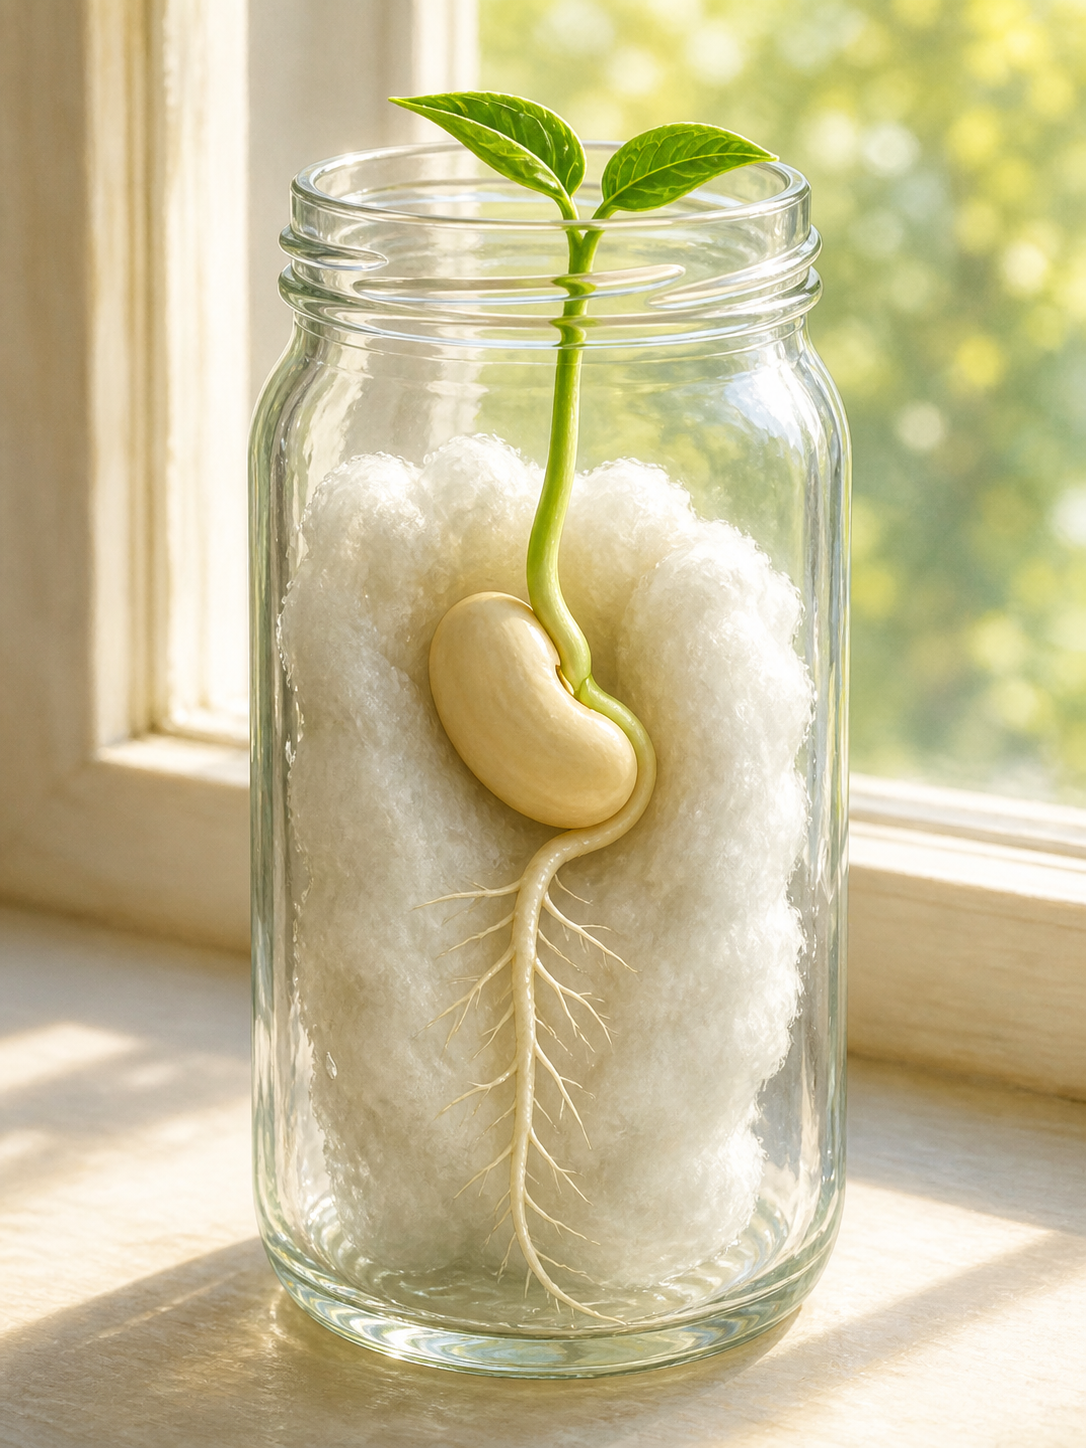
\includegraphics[width=0.44\linewidth]{images/book1/ai/g2-seed-bean-jar.png}

{\small L'expérience du bocal en pleine \omterm{def:g2:from-seed-to-plant:germination}{germination}~: la \omterm{def:g1:plants-around-us:parts}{racine} vers
le bas, la \omterm{def:g1:plants-around-us:parts}{tige} vers le haut, et la \omterm{def:g2:from-seed-to-plant:seed}{graine} qui se vide entre les
deux.}
\end{omfigure}

\begin{remark}[Racine en bas, tige en haut --- toujours]\label{rem:g2:from-seed-to-plant:updown}
Peu importe comment le haricot est couché dans le bocal --- sur le
côté, à l'envers --- la \omterm{def:g1:plants-around-us:parts}{racine} se tourne toujours vers le bas et la
\omterm{def:g1:plants-around-us:parts}{tige} toujours vers le haut. La \omterm{prop:g2:from-seed-to-plant:cycle}{jeune pousse} ne voit rien, et pourtant
elle sait où est le haut. Les \omterm{def:g1:plants-around-us:plant}{plantes} sentent plus qu'elles ne le
montrent.
\end{remark}

\section{De la jeune pousse à la plante à graines}

\begin{proposition}[Le cycle de vie de la plante]\label{prop:g2:from-seed-to-plant:cycle}
La \emph{jeune pousse}\index{jeune pousse} devient une \omterm{def:g1:plants-around-us:plant}{plante} avec
\omterm{def:g1:plants-around-us:parts}{racines}, \omterm{def:g1:plants-around-us:parts}{tige} et \omterm{def:g1:plants-around-us:parts}{feuilles}~; la \omterm{def:g1:plants-around-us:plant}{plante} fleurit~; les \omterm{def:g1:plants-around-us:parts}{fleurs} font de
nouvelles \emph{\omterm{def:g2:from-seed-to-plant:seed}{graines}}~; et le cycle peut recommencer. Un seul pied
de haricot peut faire des dizaines de nouveaux haricots en un été.
\end{proposition}
\admitted

\begin{example}[Un haricot, un été]\label{ex:g2:from-seed-to-plant:summer}
Semé en mai, un haricot germe en une semaine~; en juin, c'est une
\omterm{def:g1:plants-around-us:plant}{plante} feuillue qui grimpe le long de son tuteur~; en juillet
viennent les \omterm{def:g1:plants-around-us:parts}{fleurs} blanches, puis les cosses vertes~; en août les
cosses pendent, lourdes, chacune tenant une rangée de nouveaux
haricots --- les \omterm{def:g2:from-seed-to-plant:seed}{graines} de l'an prochain, faites par la \omterm{def:g1:plants-around-us:plant}{plante} de
cette année.
\end{example}

\section{Exercices}

\begin{exercise}[$\star$]\label{exo:g2:from-seed-to-plant:1}
Quelles deux choses se trouvent sous l'enveloppe d'une \omterm{def:g2:from-seed-to-plant:seed}{graine}~?
\end{exercise}

\begin{exercise}[$\star$]\label{exo:g2:from-seed-to-plant:2}
Que veut dire \emph{\omterm{def:g2:from-seed-to-plant:germination}{germer}}~? Qu'est-ce qui sort de la \omterm{def:g2:from-seed-to-plant:seed}{graine} en
premier~: la \omterm{def:g1:plants-around-us:parts}{racine} ou la \omterm{def:g1:plants-around-us:parts}{tige}~?
\end{exercise}

\begin{exercise}[$\star$]\label{exo:g2:from-seed-to-plant:3}
Nomme les deux choses dont une \omterm{def:g2:from-seed-to-plant:seed}{graine} a besoin pour \omterm{def:g2:from-seed-to-plant:germination}{germer}. Quel
besoin célèbre des \omterm{def:g1:plants-around-us:plant}{plantes} adultes n'est \emph{pas} dans la liste~?
\end{exercise}

\begin{exercise}[$\star$]\label{exo:g2:from-seed-to-plant:4}
Comment une \omterm{prop:g2:from-seed-to-plant:cycle}{jeune pousse} enterrée peut-elle grandir dans le noir,
avant d'atteindre la lumière~? D'où vient sa nourriture au début~?
\end{exercise}

\begin{exercise}[$\star$]\label{exo:g2:from-seed-to-plant:5}
Nomme quatre \omterm{def:g2:from-seed-to-plant:seed}{graines} que tu pourrais trouver dans une cuisine.
\end{exercise}

\begin{exercise}[$\star$]\label{exo:g2:from-seed-to-plant:6}
Pourquoi les jardiniers sèment-ils au printemps plutôt qu'en hiver~?
\end{exercise}

\begin{exercise}[$\star$]\label{exo:g2:from-seed-to-plant:7}
Range dans l'ordre~: cosse pleine de nouveaux haricots --- \omterm{def:g2:from-seed-to-plant:seed}{graine}
--- \omterm{def:g1:plants-around-us:plant}{plante} en \omterm{def:g1:plants-around-us:parts}{fleur} --- \omterm{prop:g2:from-seed-to-plant:cycle}{jeune pousse} --- \omterm{def:g1:plants-around-us:plant}{plante} feuillue.
\end{exercise}

\begin{exercise}[$\star$]\label{exo:g2:from-seed-to-plant:8}
À toi d'essayer~: monte le bocal de
\cref{met:g2:from-seed-to-plant:sow} avec deux haricots --- l'un
couché sur le côté, l'autre à l'envers. Après la \omterm{def:g2:from-seed-to-plant:germination}{germination},
compare leurs \omterm{def:g1:plants-around-us:parts}{racines} et leurs \omterm{def:g1:plants-around-us:parts}{tiges}. Que prévoit
\cref{rem:g2:from-seed-to-plant:updown}~?
\end{exercise}

\begin{exercise}[$\star\star$]\label{exo:g2:from-seed-to-plant:9}
Nina garde un sachet de \omterm{def:g2:from-seed-to-plant:seed}{graines} de haricot dans un tiroir sec toute
une année, et elles germent quand même quand elle finit par les
semer. Pourquoi n'ont-elles ni poussé ni péri dans le tiroir~?
Utilise \cref{prop:g2:from-seed-to-plant:needs}.
\end{exercise}

\begin{exercise}[$\star\star$]\label{exo:g2:from-seed-to-plant:10}
Le poussin de \cref{ch:g2:animals-grow-up} grandit dans son \omterm{def:g2:animals-grow-up:born}{œuf},
nourri par le jaune. Qu'est-ce qui joue le rôle du jaune dans un
haricot~? Qu'ont en commun un \omterm{def:g2:animals-grow-up:born}{œuf} et une \omterm{def:g2:from-seed-to-plant:seed}{graine}~?
\end{exercise}
